
% ===========================================================================
% Title:
% ---------------------------------------------------------------------------
% to create Type I fonts type "dvips -P cmz -t letter <filename>"
% ===========================================================================
\documentclass[11pt]{article}       %--- LATEX 2e base
\usepackage{latexsym}               %--- LATEX 2e base
%---------------- Wide format -----------------------------------------------
\textwidth=6in \textheight=9in \oddsidemargin=0.25in
\evensidemargin=0.25in \topmargin=-0.5in
%--------------- Algorithm --------------------------------------------------
\newtheorem{algX}{Algorithm}
\newenvironment{algorithm}       {\begin{algX}\begin{em}}%
                                 {\par\noindent --- End of Algorithm ---
                                 \end{em}\end{algX}}
\newcommand{\step}[2]            {\begin{list}{}
                                  {  \setlength{\topsep}{0cm}
                                     \setlength{\partopsep}{0cm}
                                     \setlength{\leftmargin}{0.8cm}
                                     \setlength{\labelwidth}{0.7cm}
                                     \setlength{\labelsep}{0.1cm}    }
                                  \item[#1]#2    \end{list}}
                                 % usage: \begin{algorithm} \label{xyz}
                                 %        ... \step{(1)}{...} ...
                                 %        \end{algorithm}
%--------------- Figures ----------------------------------------------------
\usepackage{graphicx}

\newcommand{\includeFig}[3]      {\begin{figure}[htb] \begin{center}
                                 \includegraphics
                                 [width=4in,keepaspectratio]
                                 {#2}\caption{\label{#1}#3} \end{center} \end{figure}}
                                 % usage: \includeFig{label}{file}{caption}


% ===========================================================================
\begin{document}
% ===========================================================================

% ############################################################################
% Title
% ############################################################################

\title{Accelerating Genetic ANN Training using the CUDA Platform}


% ############################################################################
% Author(s) (no blank lines !)
\author{
% ############################################################################
Catalin Patulea and Robert Peace\\
School of Systems and Computer Engineering\\
Carleton University\\
Ottawa, Canada K1S 5B6\\
{\em rpeace@sce.carleton.ca}
% ############################################################################
} % end-authors
% ############################################################################

\maketitle

% ############################################################################
% Abstract
% ############################################################################
\begin{abstract}
We present an implementation of genetic algorithm (GA) training of artificial neural networks (ANNs) targeting commodity graphics cards (GPUs). By carefully mapping the problem onto the unique GPU architecture, we achieve order-of-magnitude speedup over a conventional CPU implementation. Furthermore, we show that the speedup is consistent across a wide range of population and training set sizes. This performance boost enables classifier design to span a wider range of population sizes and number of generations affording better classifiers and improved understanding of long-term trends in genetic algorithm convergence. Finally, we apply this method to the design of a classifier for the 2009 UC San Diego Data Mining Contest.
\end{abstract}

% ############################################################################
\section{Introduction} \label{intro}
% ############################################################################

% ############################################################################
\section{Background} \label{background}
% ############################################################################

% ----------------------------------------------------------------------------
\subsection{Artificial Neural Networks} \label{ann}
% ----------------------------------------------------------------------------
Artificial neural networks (ANNs) are very flexible classifiers. By varying the network structure and parameters thereof, they can represent many aspects of the function to be approximated, including nonlinearities and high-order terms. However, the complexity of these classifiers implies that finding optimal parameters coincides with a search in a very high-dimensional parametric space. This is known as an optimization problem, for which a wide variety of solutions are known.

Greedy approaches to ANN training include gradient descent, Gauss-Newton and Levenberg�Marquardt, which are first order, second order and hybrid methods, respectively. These methods seek extrema using the local behaviour of the error function and are thus susceptible to getting stuck at local extrema rather than finding the global extremum.

Stochastic approaches offer the promise of "eventually" reaching the global extremum by asymptotically exploring the entire search space. Simulated annealing, for example, iteratively generates candidate solutions by randomly perturbing the previous solution. Early in the process, we inject a high amount of randomness to find global trends in the error function, while later in the process we inject less randomness to find the apex of the (hopefully) global extremum.

% ----------------------------------------------------------------------------
\subsection{Genetic Algorithms} \label{ga}
% ----------------------------------------------------------------------------
Genetic algorithms (GAs) rely on multiple candidate solutions to simultaneously explore the search space. The "individuals" are randomly mutated, mated and selected during each of several generations. Mutation and mating is done using problem-specific representation of candidate solutions and "genetic operators", while selection is governed by a fitness function (classifier performance). The competitive bias imposed by selection attempts to mimic the "survival of the fittest" principle so often seen in Nature.

GA training of ANNs is very computationally-intensive. For each generation ($10^1$--$10^2$) individuals), the fitness of each individual is calculated by applying each neural network to the entire training set ($10^2$--$10^6$ instances) and taking the classification accuracy for that network. Each ANN evaluation itself requires a large number of multiplications (which increases with the number of features and hidden nodes) in addition to evaluation of transcendentals for the most commonly-used node activation function. Thus, a CPU implementation of GA training of ANNs for any but the smallest networks and training sets is infeasible.

% ----------------------------------------------------------------------------
\subsection{The CUDA Platform} \label{cuda}
% ----------------------------------------------------------------------------

Compute Unified Device Architecture (CUDA) is a platform which enables the use of NVIDIA graphics cards (GPUs) for general purpose programming, including scientific computations. GPUs have recently become quite affordable to the point that some new notebook computers now include built-in GPUs. Because of the nature of graphics processing, these are massively parallel processors optimized for memory bandwidth and floating-point computation. This is a very good match for our GA-ANN training problem.

The CUDA programming model is designed to allow algorithms to scale with the GPU's parallelism parameters. This allows the same algorithm to run on different present-day hardware as well as future hardware, with minimal changes. However, to accomplish this, the programming model is different in many ways from the conventional CPU programming. In particular, to best leverage GPU hardware, CUDA code must be carefully written to balance mathematical operations with memory accesses and to have certain specific optimal memory access patterns. These are both well-known problems in high performance computing, but they are further exacerbated by the design of the CUDA architecture.


% ############################################################################
\section{Methods} \label{algimp}
% ############################################################################
Filling this with text so that I can see what the document looks like when it is filled with text and to make sure that everything lines up nicely when it is full of text like this

% ----------------------------------------------------------------------------
\subsection{Preliminary Data Analysis} \label{prelim}
% ----------------------------------------------------------------------------
Filling this with text so that I can see what the document looks like when it is filled with text and to make sure that everything lines up nicely when it is full of text like this

% ----------------------------------------------------------------------------
\subsection{Data Preprocessing Steps} \label{preprocessing}
% ----------------------------------------------------------------------------
Filling this with text so that I can see what the document looks like when it is filled with text and to make sure that everything lines up nicely when it is full of text like this

% ----------------------------------------------------------------------------
\subsection{Classifier Design} \label{design}
% ----------------------------------------------------------------------------
Filling this with text so that I can see what the document looks like when it is filled with text and to make sure that everything lines up nicely when it is full of text like this

% ----------------------------------------------------------------------------
\subsection{Classifier Implementation} \label{implementation}
% ----------------------------------------------------------------------------
Filling this with text so that I can see what the document looks like when it is filled with text and to make sure that everything lines up nicely when it is full of text like this

% ############################################################################
\section{Results} \label{results}
% ############################################################################
Filling this with text so that I can see what the document looks like when it is filled with text and to make sure that everything lines up nicely when it is full of text like this

% ----------------------------------------------------------------------------
\subsection{Experimental Setup} \label{experiment}
% ----------------------------------------------------------------------------
To evaluate the performance of our system, we compared execution time of equivalent algorithms running on commodity desktop CPUs and GPUs. Each series represents one type of experimental hardware (Table~\ref{tab:experimental-hardware}). Each data point is an average over 10 runs of the algorithm with the same parameters.

\begin{table}
	\centering
	\begin{tabular}{ll}
	\textbf{Legend Label} & \textbf{Hardware} \\
	\hline
	Core2 & Intel Core 2 Q9450 CPU at 2.66 GHz \\
	GTX275 & NVidia GTX275 GPU \\
	\hline
	\end{tabular}
	\caption{Experimental hardware}
	\label{tab:experimental-hardware}
\end{table}

% ----------------------------------------------------------------------------
\subsection{Performance Results} \label{performance}
% ----------------------------------------------------------------------------
In most cases, the GPU implementation resulted in approximately an order of magnitude speedup over a CPU implementation (Figure~\ref{fig:training-performance}). For low population sizes, GPU initialization and data copying dominates.

\begin{figure}
	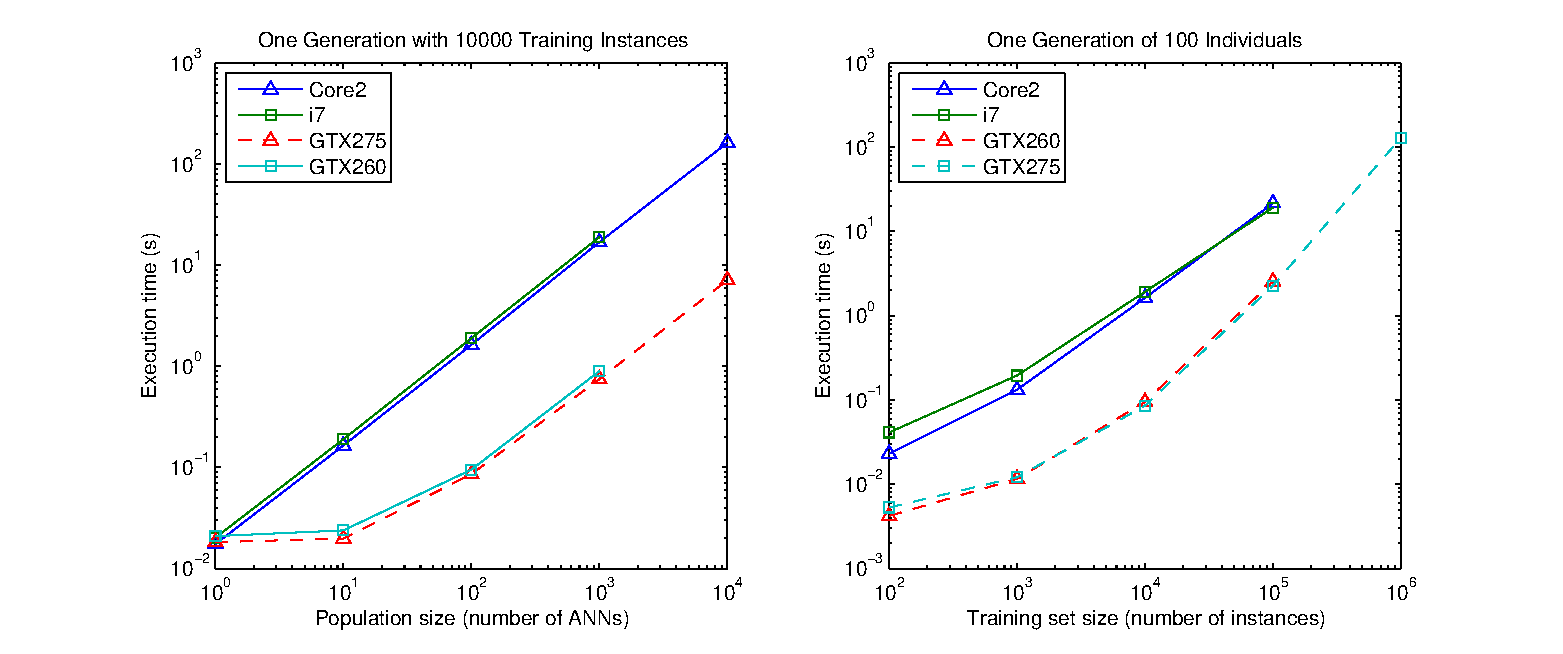
\includegraphics[width=\textwidth]{fig-performance}
	\caption{Training performance as a function of population size (left) and training set size (right). Note logarithmic axes.}
	\label{fig:training-performance}
\end{figure}

% ----------------------------------------------------------------------------
\subsection{Classifier Results} \label{results}
% ----------------------------------------------------------------------------
Filling this with text so that I can see what the document looks like when it is filled with text and to make sure that everything lines up nicely when it is full of text like this

% ############################################################################
\section{Conclusion} \label{concl}
% ############################################################################
Filling this with text so that I can see what the document looks like when it is filled with text and to make sure that everything lines up nicely when it is full of text like this

% ############################################################################
\section{Discussion} \label{disc}
% ############################################################################
Filling this with text so that I can see what the document looks like when it is filled with text and to make sure that everything lines up nicely when it is full of text like this

% ----------------------------------------------------------------------------
\subsection{Future Work} \label{future}
% ----------------------------------------------------------------------------
Filling this with text so that I can see what the document looks like when it is filled with text and to make sure that everything lines up nicely when it is full of text like this

% ############################################################################
% Bibliography
% ############################################################################
\bibliographystyle{plain}
\bibliography{bibliography}     %loads bibliography.bib

% ============================================================================
\end{document}
% ============================================================================
